\subsection{Descripci\'on del algoritmo}

Como algoritmo exacto para resolver el problema se eligi\'o la t\'ecnica de programaci\'on Backtracking, la cual recorre todas los caminos posibles de $u$ a $v$, realizando a su vez podas para mejorar la $performance$ (el mismo puede encontrarse en la p\'agina siguiente).\\\\

Iniciamos el algoritmo creando una variable para guardar el mejor camino encontrado hasta el momento, que guarda la suma de $w_{1}$ y $w_{2}$ del camino para poder comparar con otros. Tambi\'en inicializamos otra variable para ir armando el camino que se va generando en cada llamada recursiva.\\

El problema comienza a ser resuelto con la primera llamada a la funci\'on $backtrack$ a la cual se le pasa por par\'ametro el grafo para el que se debe buscar el camino, el nodo de destino, la cota $K$, un arreglo para controlar los nodos que ya fueron visitados (para no entrar en un $loop$) y las referencias al camino actual y al mejor camino encontrado.
\\

Siguiendo con la t\'ecnica de Backtracking, la idea es tomar un nodo y recorrer todos los caminos posibles por cada nodo adyacente de manera recursiva, es decir, comenzamos por el nodo source, en este caso $u$, para cada uno de sus nodos adyacentes abrimos una rama que va a intentar llegar al nodo target, $v$ para nosotros, abriendo nuevas ramas a trav\'es de sus nodos adyacentes. Repitiendo recursivamente este procedimiento, logramos obtener todas los caminos de $u$ a $v$ posibles, quedandonos con el de menor costo en $w_{2}$ de los acotados por $K$.

\newpage
\subsection{Algoritmo}

\lstset{language=C++,
                basicstyle=\ttfamily\footnotesize,
                keywordstyle=\color{blue}\ttfamily,
                stringstyle=\color{red}\ttfamily,
                commentstyle=\color{green}\ttfamily,
                morecomment=[l][\color{magenta}]{\#},
                breaklines=true
}
\begin{lstlisting}
struct Camino{
	list<int> * camino;
	double w1_total;
	double w2_total;
};

// Estructura que guarda el mejor camino que encontre cumpliendo ambas condiciones
Camino mejorcamino = Camino();
mejorcamino.camino = new list<int>();
mejorcamino.w1_total = 0;
mejorcamino.w2_total = INFINITY;

// El camino que voy construyendo en cada rama del backtracking, siempre arranca desde u
Camino camino_actual = Camino();
camino_actual.camino = new list<int>();
(*camino_actual.camino).push_back(u);
camino_actual.w1_total = 0.0;
camino_actual.w2_total = 0.0;
vector<bool> * nodos_visitados = new vector<bool>(n+1, false);
(*nodos_visitados)[u] = true;
		
backtrack(grafo, v, k, nodos_visitados, camino_actual, mejorcamino);

void backtrack(graph * grafo, int nodo_objetivo, double k, vector<bool> * nodos_visitados, Camino & camino_actual, Camino & mejor_camino) {
	
	int ultimo_nodo = (*camino_actual.camino).back(); // Ultimo nodo agregado
	list<int> * nodos_adyacentes = grafo->get_adyacentes(ultimo_nodo); // Nodos adyacentes al ultimo nodo recorrido
	
	// Si me pase de la cota K corto esta rama
	if(camino_actual.w1_total > k){
		return;
	}
	
	// Si ya encontre el nodo final termino
	if(ultimo_nodo == nodo_objetivo){

		if(camino_actual.w2_total < mejor_camino.w2_total){
			delete mejor_camino.camino;
			mejor_camino.camino = new list<int>((*camino_actual.camino));
			mejor_camino.w1_total = camino_actual.w1_total;
			mejor_camino.w2_total = camino_actual.w2_total;
		}
		return;
	}
	
	// Recorro los adyancentes del ultimo nodo recorrido
	for(list<int>::iterator nodo = nodos_adyacentes->begin(); nodo != nodos_adyacentes->end(); nodo++){
		// Si ya visite el nodo termino
		if((*nodos_visitados)[*nodo] == true){
			continue;
		}

		(*nodos_visitados)[*nodo] = true; // Marco el nodo como visitado para hacer el llamado recursivo
		(*camino_actual.camino).push_back(*nodo);
		camino_actual.w1_total = camino_actual.w1_total + grafo->get_w1(ultimo_nodo, *nodo);
		camino_actual.w2_total = camino_actual.w2_total + grafo->get_w2(ultimo_nodo, *nodo);
		
		backtrack(grafo, nodo_objetivo, k, nodos_visitados, camino_actual, mejor_camino);
		// Restauro el estado para cuando vuelva
		camino_actual.w1_total = camino_actual.w1_total - grafo->get_w1(ultimo_nodo, *nodo);
		camino_actual.w2_total = camino_actual.w2_total - grafo->get_w2(ultimo_nodo, *nodo);
		(*nodos_visitados)[*nodo] = false;
		(*camino_actual.camino).pop_back();		
	}
}
\end{lstlisting}

\newpage
\subsection{An\'alisis de complejidad}

Para este punto debemos indicar la complejidad del algoritmo en el peor caso, para esto es necesario primero identificar que ser\'ia un peor caso.
Analizando el funcionamiento del backtracking, el comportamiento se orienta hacia el peor caso si en cada paso se abren la mayor cantidad de ramas, por lo tanto esto nos lleva a pensar que el peor caso ser\'a un grafo completo, ya que al estar todos los nodos conectados contra todos, en primera instancia recorreremos $n-1$ ramas, correspondientes a los $n-1$ nodos adyacentes al nodo source, luego cada una de estas se abrir\'a a los $n-2$ nodos adyacentes restantes a los que se puede conectar cada uno y as\'i sucesivamente. En este sentido la complejidad del peor caso ser\'ia O($(n-1)!$), acotado asint\'oticamente por O($n!$).

Veamos entonces gr\'aficamente el comportamiento del algoritmo:

\subsection{Gr\'afico de complejidad}
\begin{figure}[!hp]
	\centering
 	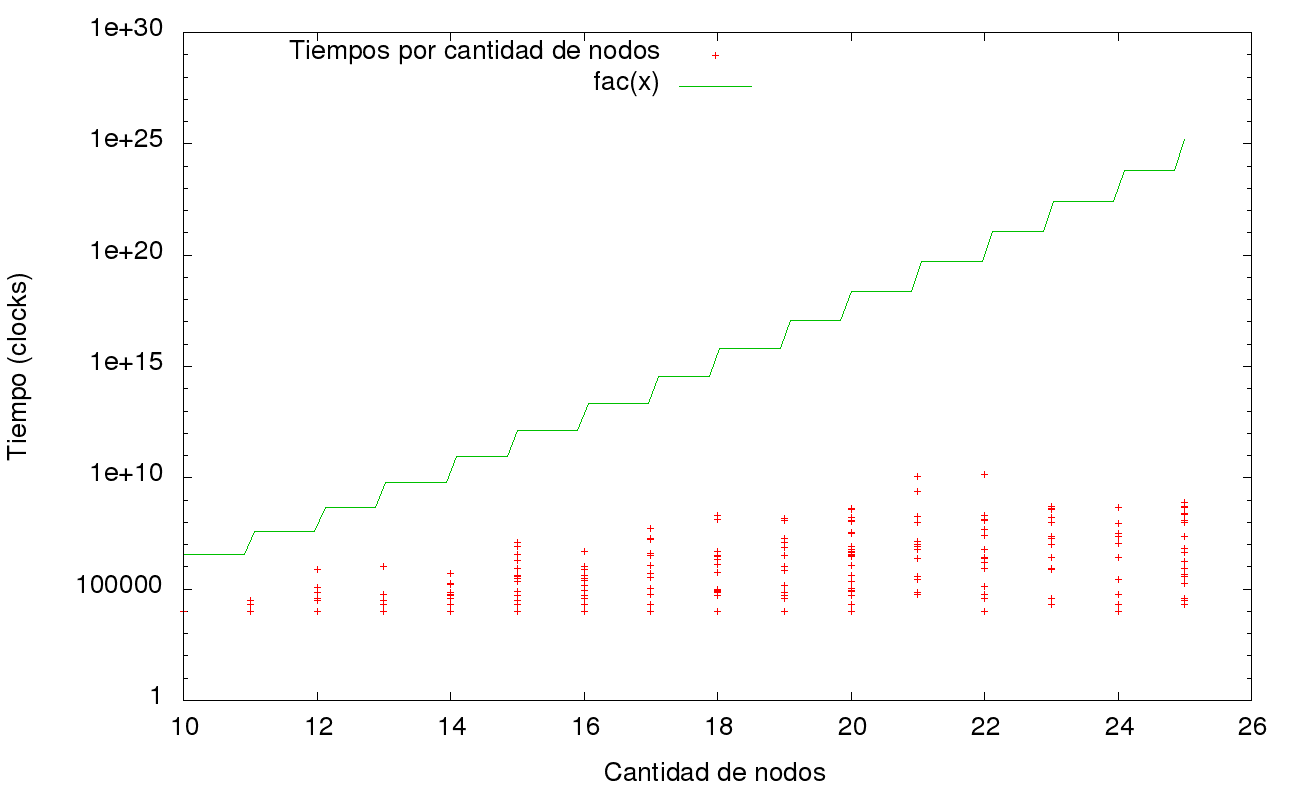
\includegraphics[scale=0.3]{img/exacto_time.png}
\end{figure}

M\'as all\'a de la escala logar\'itmica, podemos apreciar que el comportamiento es el esperado, es deir que los tiempos de ejecuci\'on son muy elevados.
Tambi\'en podemos apreciar que no necesariamente se apega a la cota de $n!$, esto se debe a que ese es el peor de los casos, cuando todos los grafos tienden a ser completos.


\subsection{Conclusiones}

A partir de la experimentaci\'on se pudo ver que un algoritmo exacto, si bien resuelve el problema, no es eficiente para un problema de estas caracter\'isticas, ya que verificar todas las soluciones posibles (incluso aunque no sean todas, ya que el backtracking descarta las que sabe que no son viables) lo hace muy lento.\\
En casos como \'este puede ser una mejor opci\'on pensar y testear distintas heur\'isticas.\\

Una heur\'istica es un algoritmo no necesariamente exacto que permite llegar a la soluci\'on de un problema en tiempo razonable, a diferencia de uno exacto como el probado m\'as arriba.\\
Pero, a diferencia de un algoritmo exacto, muchas veces la soluci\'on que se obtiene es aproximada (por eso no es necesariamente exacto). Sin embargo, la soluci\'on alcanzada puede ser suficiente en algunos casos.\\\\

Veamos a continuaci\'on implementaciones de distintos tipos de heur\'isticas para resolver el mismo problema.\\
